\subsection*{Newtonian kernels in \eqref{k2n}}
\begin{align}
F_{2}(\bm{k}_{1}, \bm{k}_{2}) &= \frac{10}{7} + {\hat{\bm{k}}_{1} \cdot \hat{\bm{k}}_2}\bigg(\frac{k_{1}}{k_{2}} + \frac{k_{2}}{k_{1}}\bigg) + \frac{4}{7}\big({\hat{\bm{k}}_{1} \cdot \hat{\bm{k}}_2}\big)^{2}\,,
\label{e18} \\
G_{2}(\bm{k}_{1}, \bm{k}_{2}) &= \frac{6}{7} + {\hat{\bm{k}}_{1} \cdot \hat{\bm{k}}_2}\bigg(\frac{k_{1}}{k_{2}} + \frac{k_{2}}{k_{1}}\bigg) + \frac{8}{7}\big({\hat{\bm{k}}_{1} \cdot \hat{\bm{k}}_2}\big)^{2} \label{e19}\,,\\
Z_2(\bm{k}_1,\bm{k}_2) &=
 f \frac{\mu_1\mu_2}{k_1k_2}\big( \mu_1k_1+\mu_2k_2\big)^2 
+ \frac{b_{1}}{k_1k_2}\Big[ \big(\mu_1^2+\mu_2^2 \big)k_1k_2+\mu_1\mu_2\big(k_1^2+k_2^2 \big) \Big]\,, \label{e16x} \\  
S_{2}(\bm{k}_{1}, \bm{k}_{2}) &= \big({\hat{\bm{k}}_{1} \cdot \hat{\bm{k}}_2}\big)^{2} - \frac{1}{3}\,. \label{e20}
\end{align}

\subsection*{Fitting formulas for Fig.~\ref{fig1} curves}
\begin{align}
b_1(z) &= 0.9+0.4 z\,, \quad b_2(z) = -0.741 - 0.125\,z + 0.123\,z^{2} + 0.00637\,z^{3}\,, \label{e9}  \\
 b_{s^2}(z) &= 0.0409 - 0.199\,z - 0.0166\,z^{2} + 0.00268\,z^{3} \,, \label{e11} \\
 V(z) &= 8.85\, z^{1.65}\exp\big({-0.777\,z}\big)~ h^{-3}\,\mathrm{Gpc}^{3}\,, \label{e11_1} \\
n_{g}(z) &= 0.0193\, z^{-0.0282}\exp\big({-2.81\,z}\big) ~h^{3}\,\mathrm{Mpc}^{-3}\,,
 \label{e11_2}\\
\sigma(z)& = \big(5.29 - 0.249\,z - 0.720\,z^{2} + 0.187\,z^{3}\big)~h^{-1}\,\mathrm{Mpc}\,. \label{e14a}
\end{align}


\subsection*{{Number of orientation bins}}


Figure~\ref{fig4x} 
shows the effect on the 
relativistic 
total SNR of changing the number of orientation bins, $n_{\mu_1}=N_{\mu_1}/\Delta{\mu_1}=2 /\Delta{\mu_1}$  and $n_\varphi=N_\varphi/\Delta\varphi =2\pi/\Delta\varphi$. It is apparent 
that reducing the number of bins increases the cumulative SNR. The cumulative SNR 
converges towards a minimum for 
$n_{\mu_{1}}\,, n_{\varphi} > 40$.
We choose $n_{\mu_{1}}= n_{\varphi}=50$, which is equivalent to \eqref{ori}.
\begin{figure}[ht]
\centering
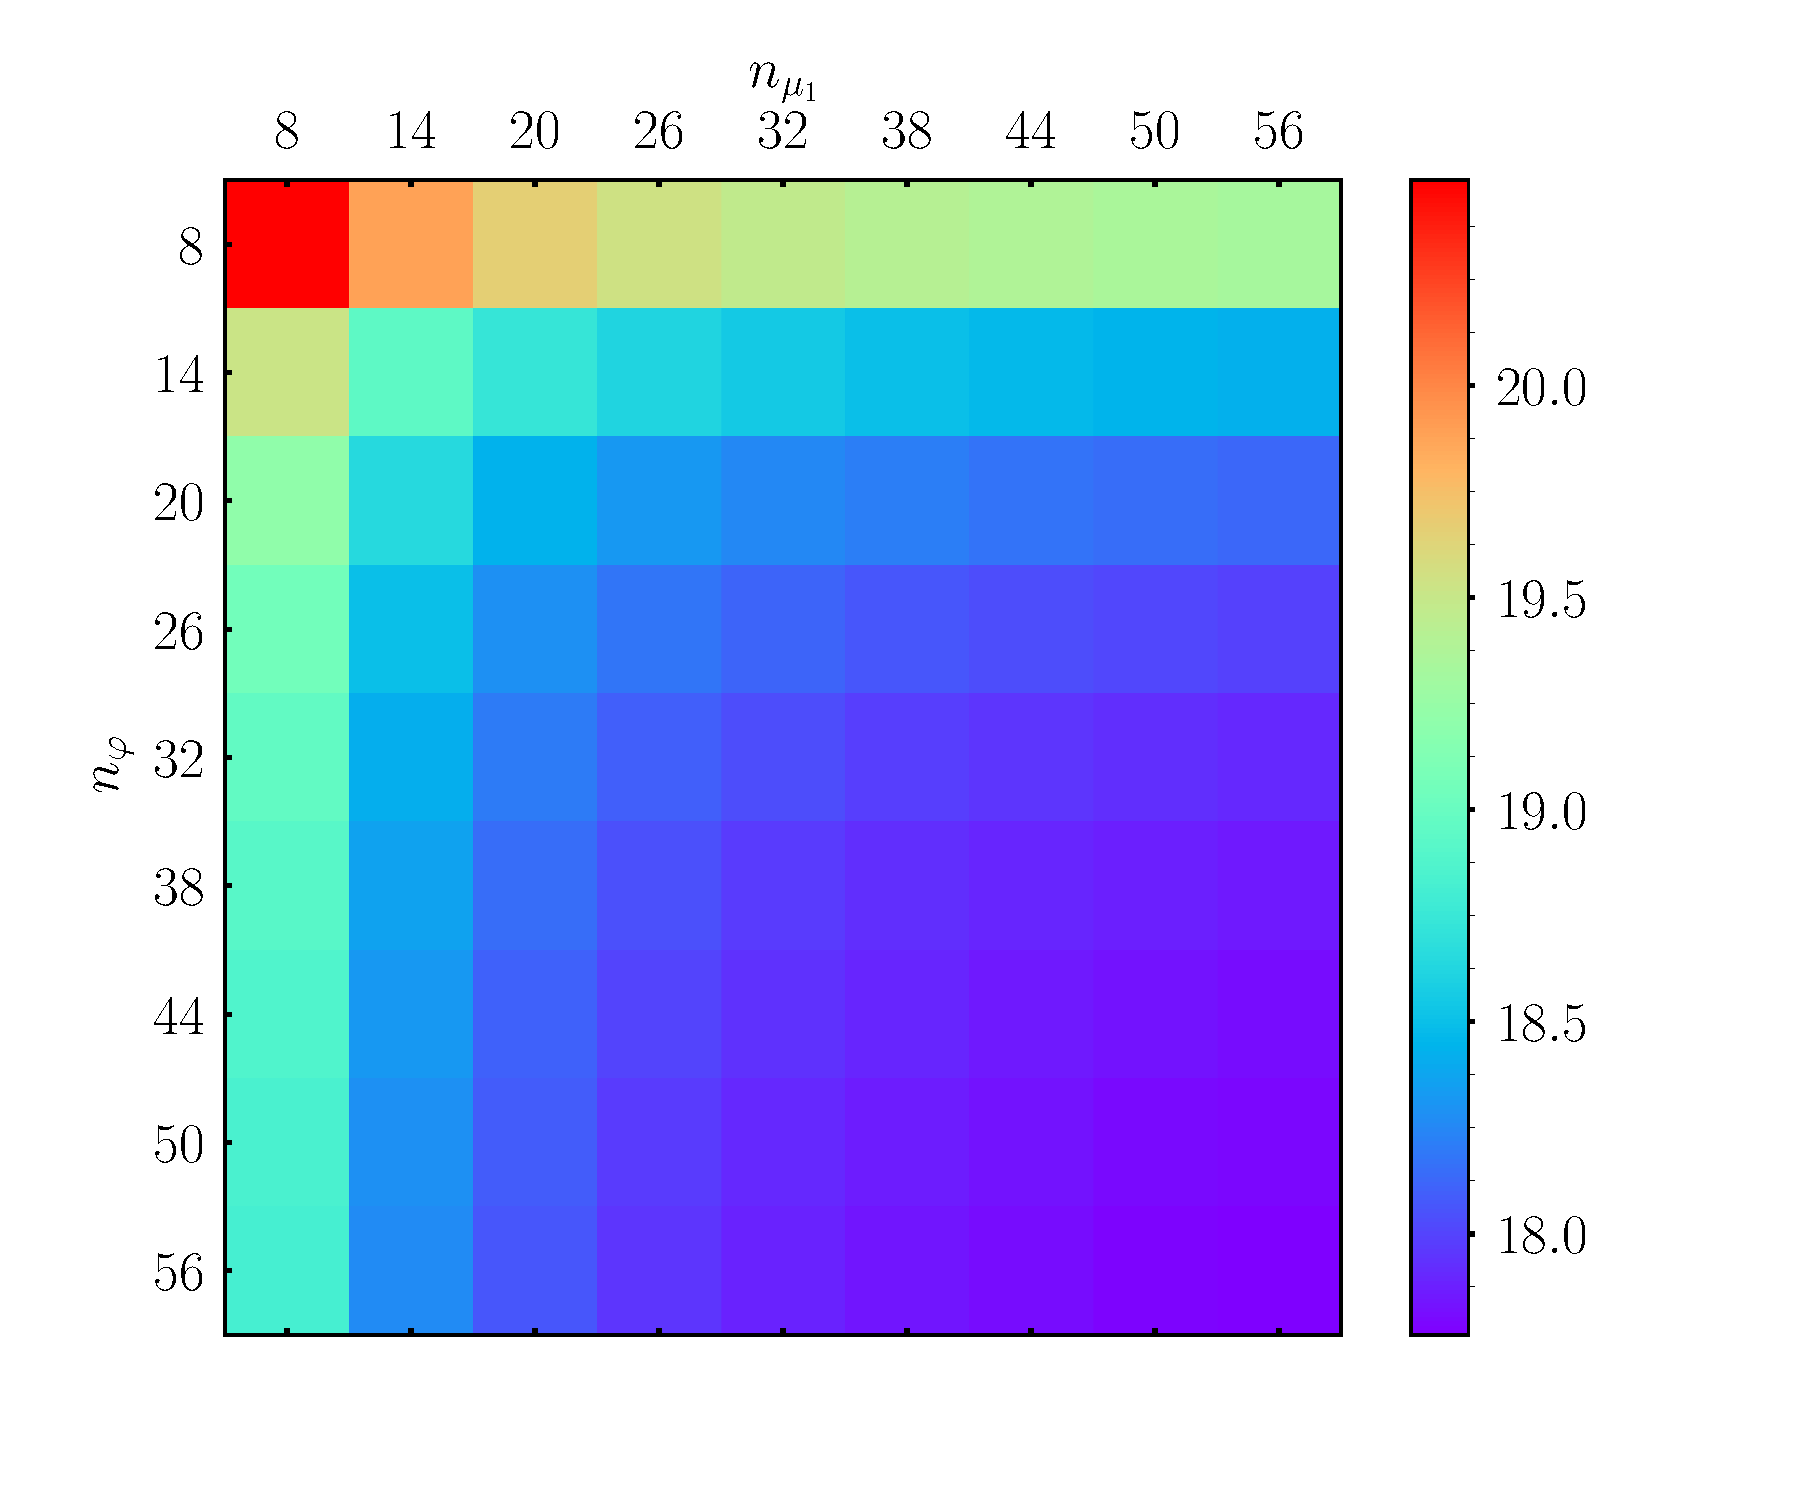
\includegraphics[width=8.0cm]{fig/colournmu1nphi_Doppler-eps-converted-to} 
\caption{Effect on 
{total} relativistic SNR of changing number of  $\varphi$ and $\mu_1$ bins. 
} \label{fig4x}
\end{figure} 


\subsection*{{Effect of changing magnification and evolution biases}}

The effect on the relativistic SNR of changes in magnification bias and in evolution bias is illustrated in Fig.~\ref{fig1x}.

\begin{figure}[ht]
\centering
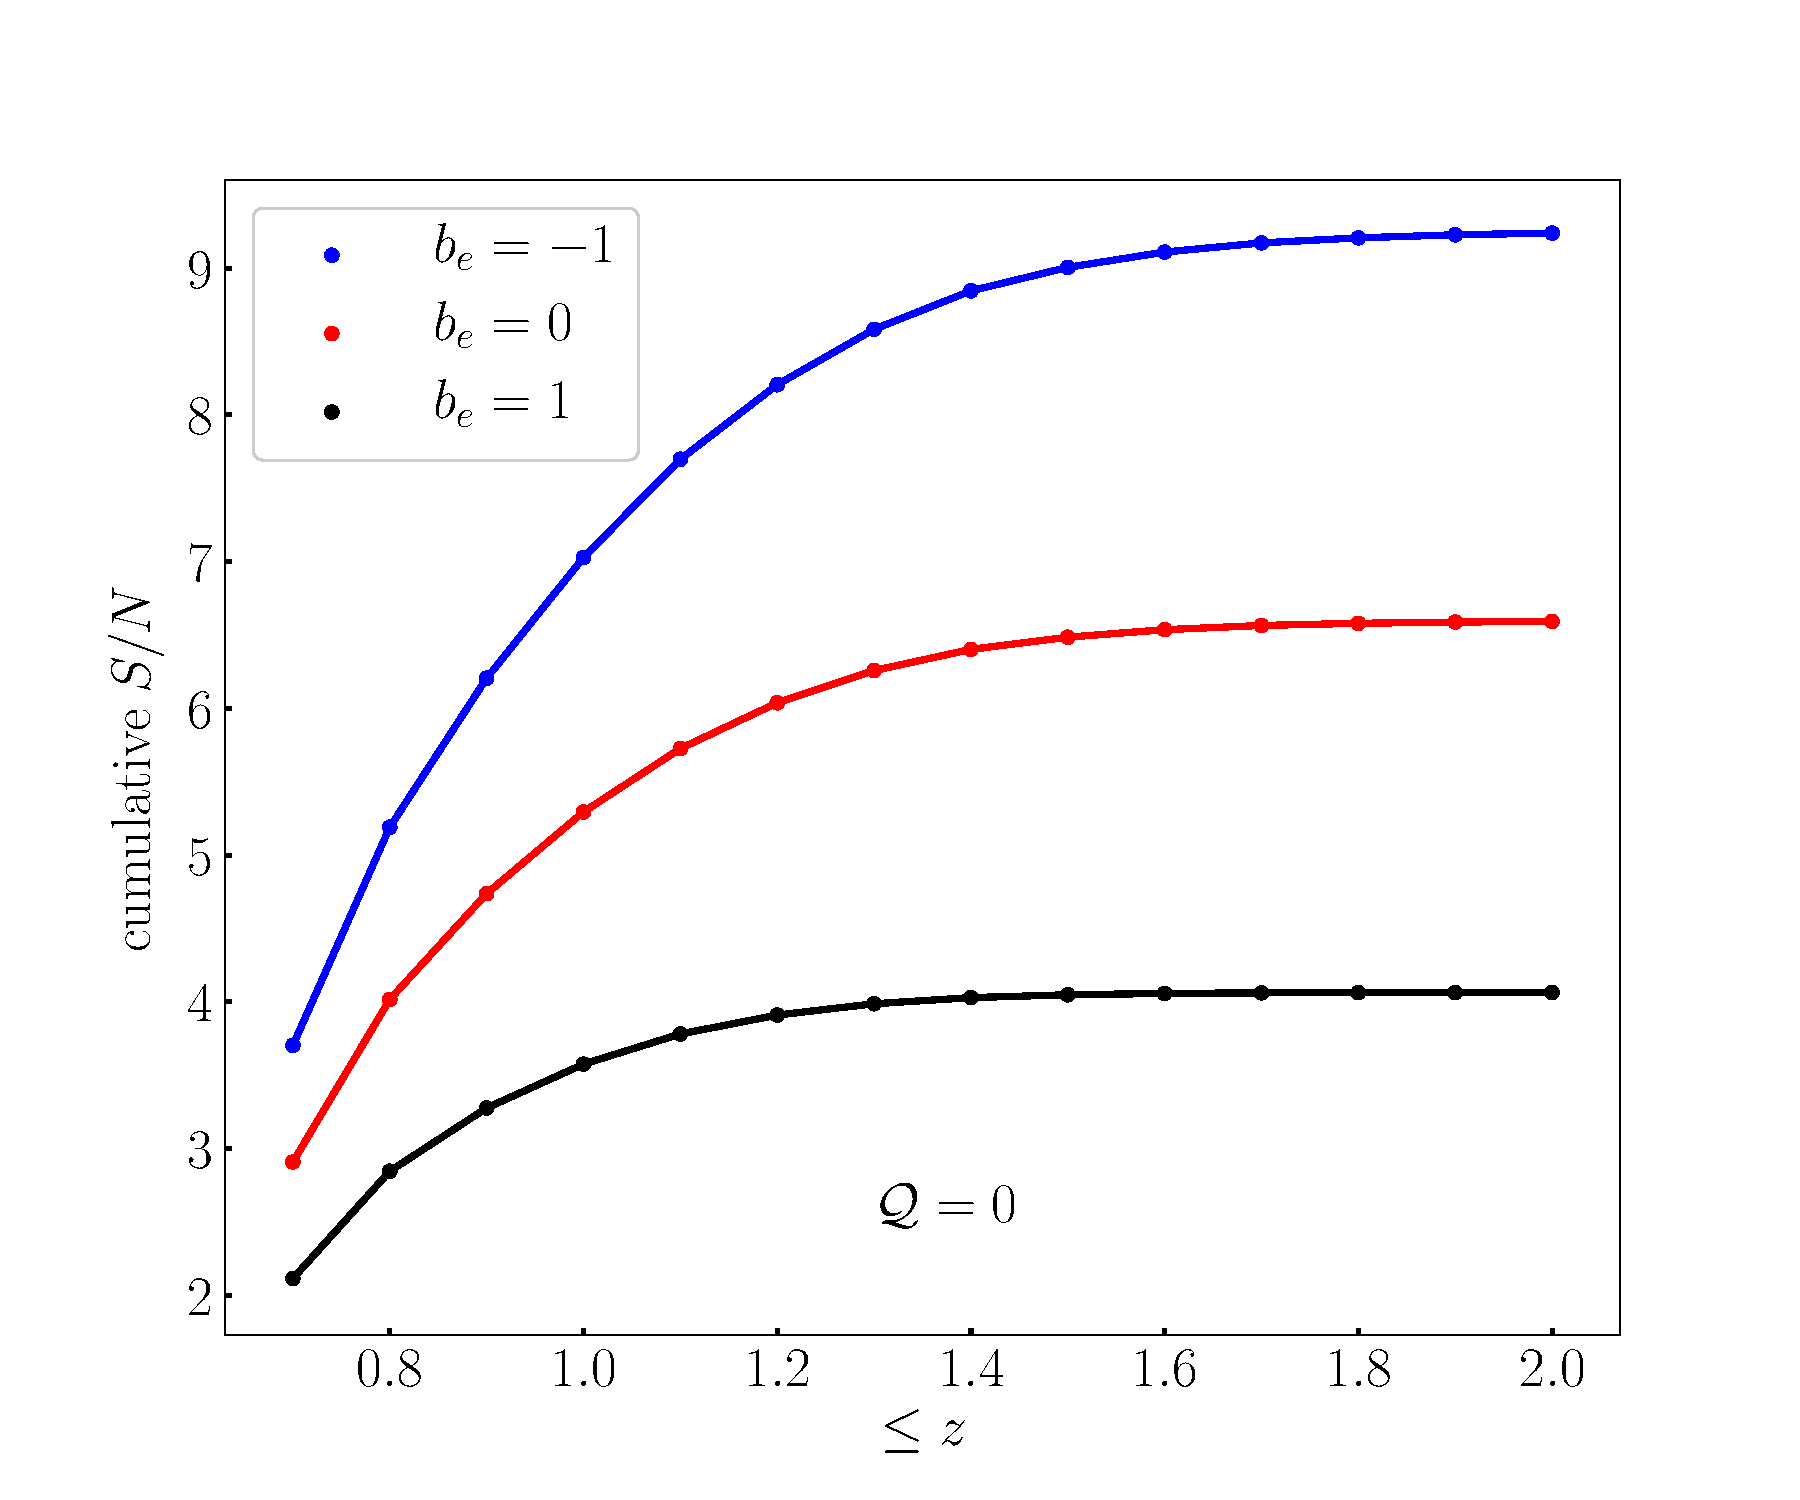
\includegraphics[width=7cm]{fig/cumulativeSnrdopplerQ0_0-eps-converted-to} 
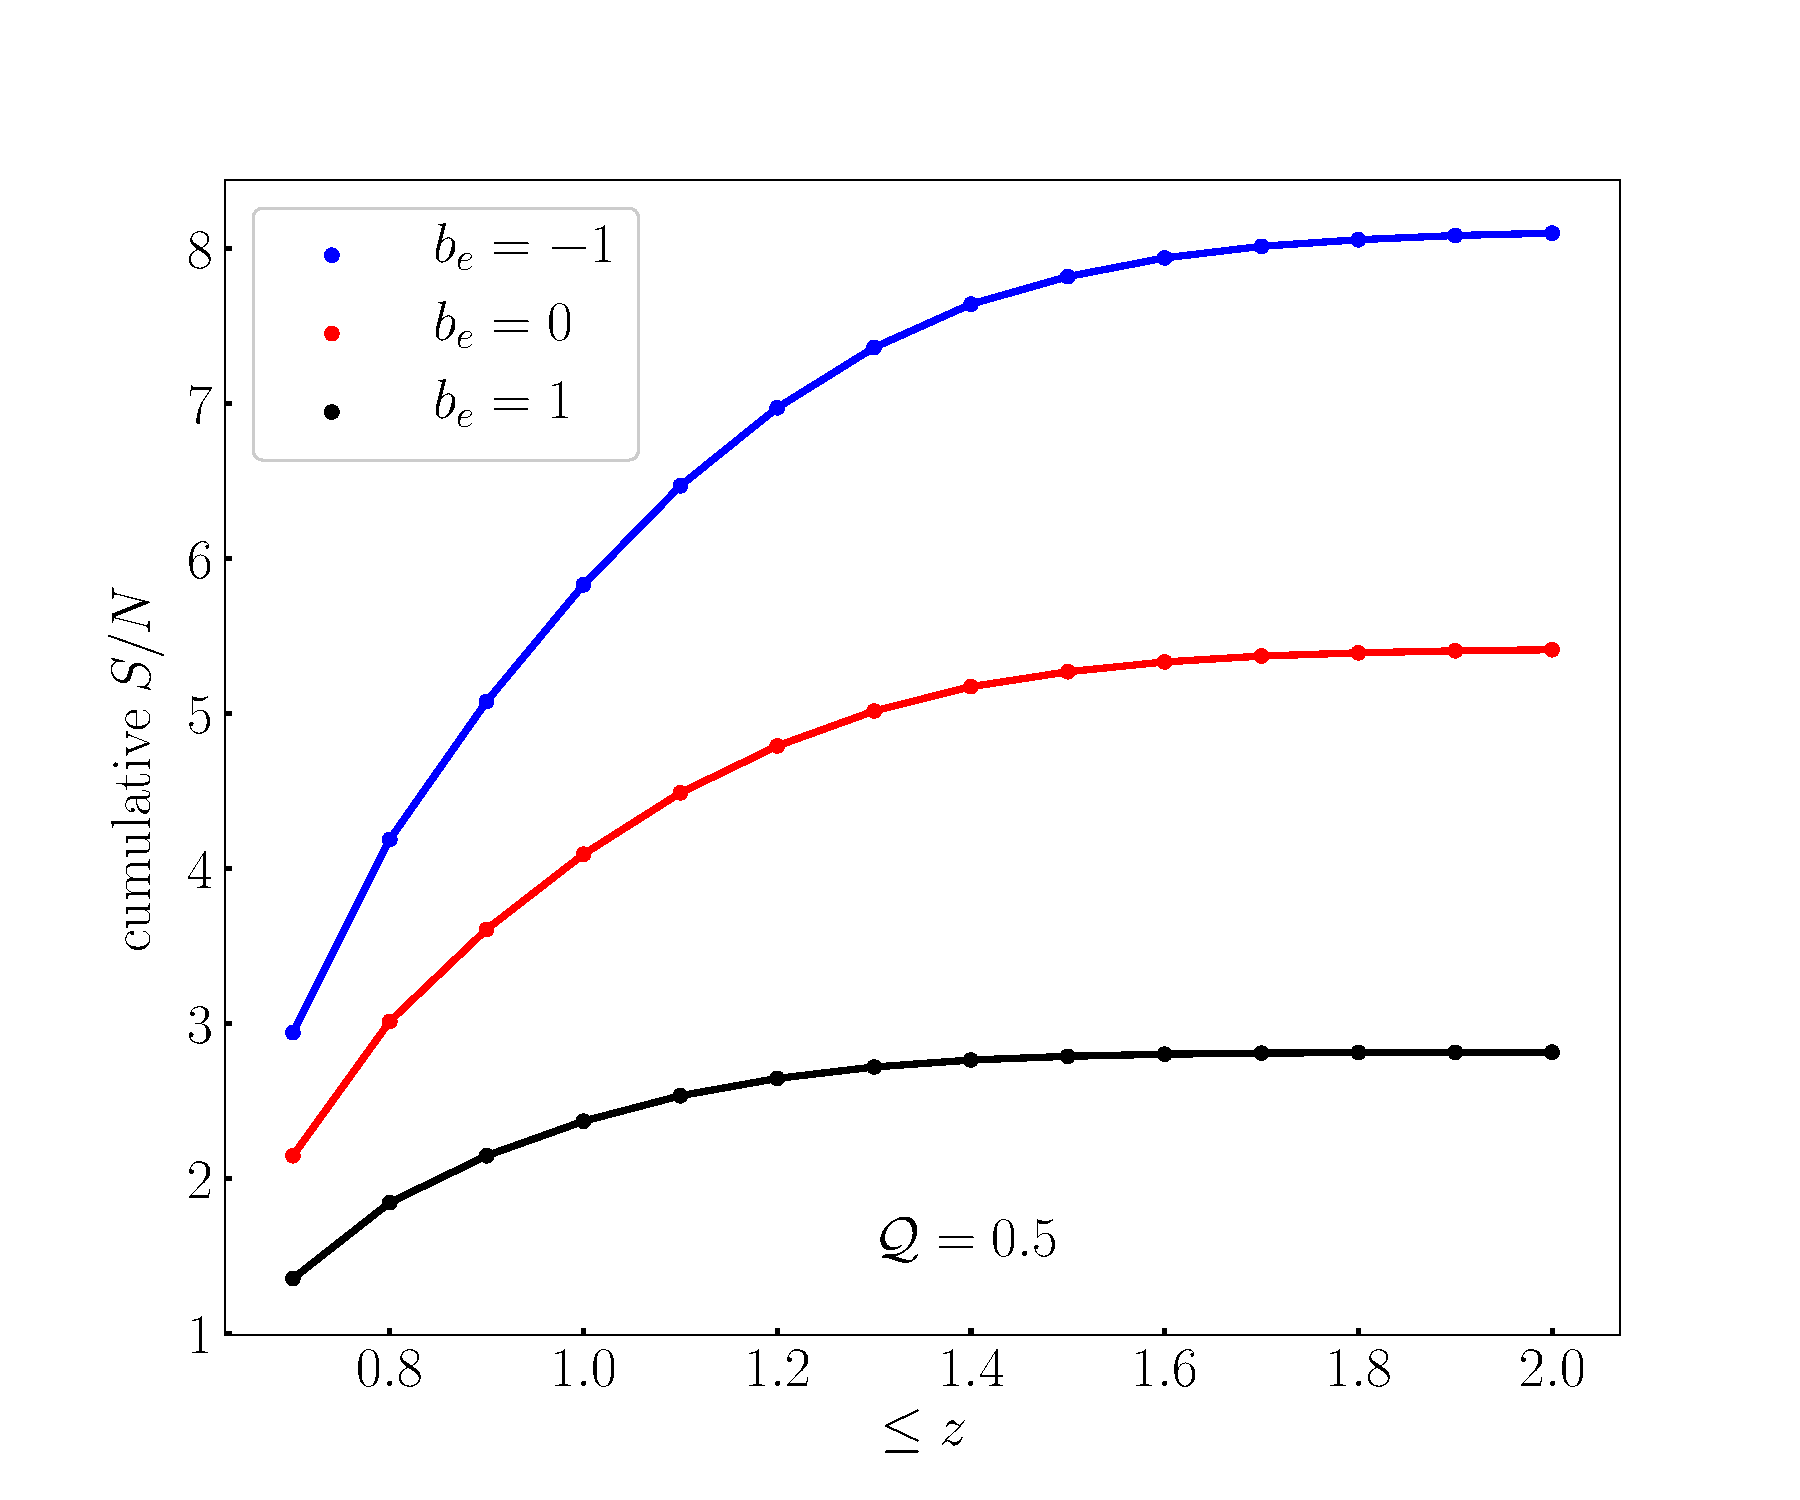
\includegraphics[width=7cm]{fig/cumulativeSnrdopplerQ0_5-eps-converted-to} \\
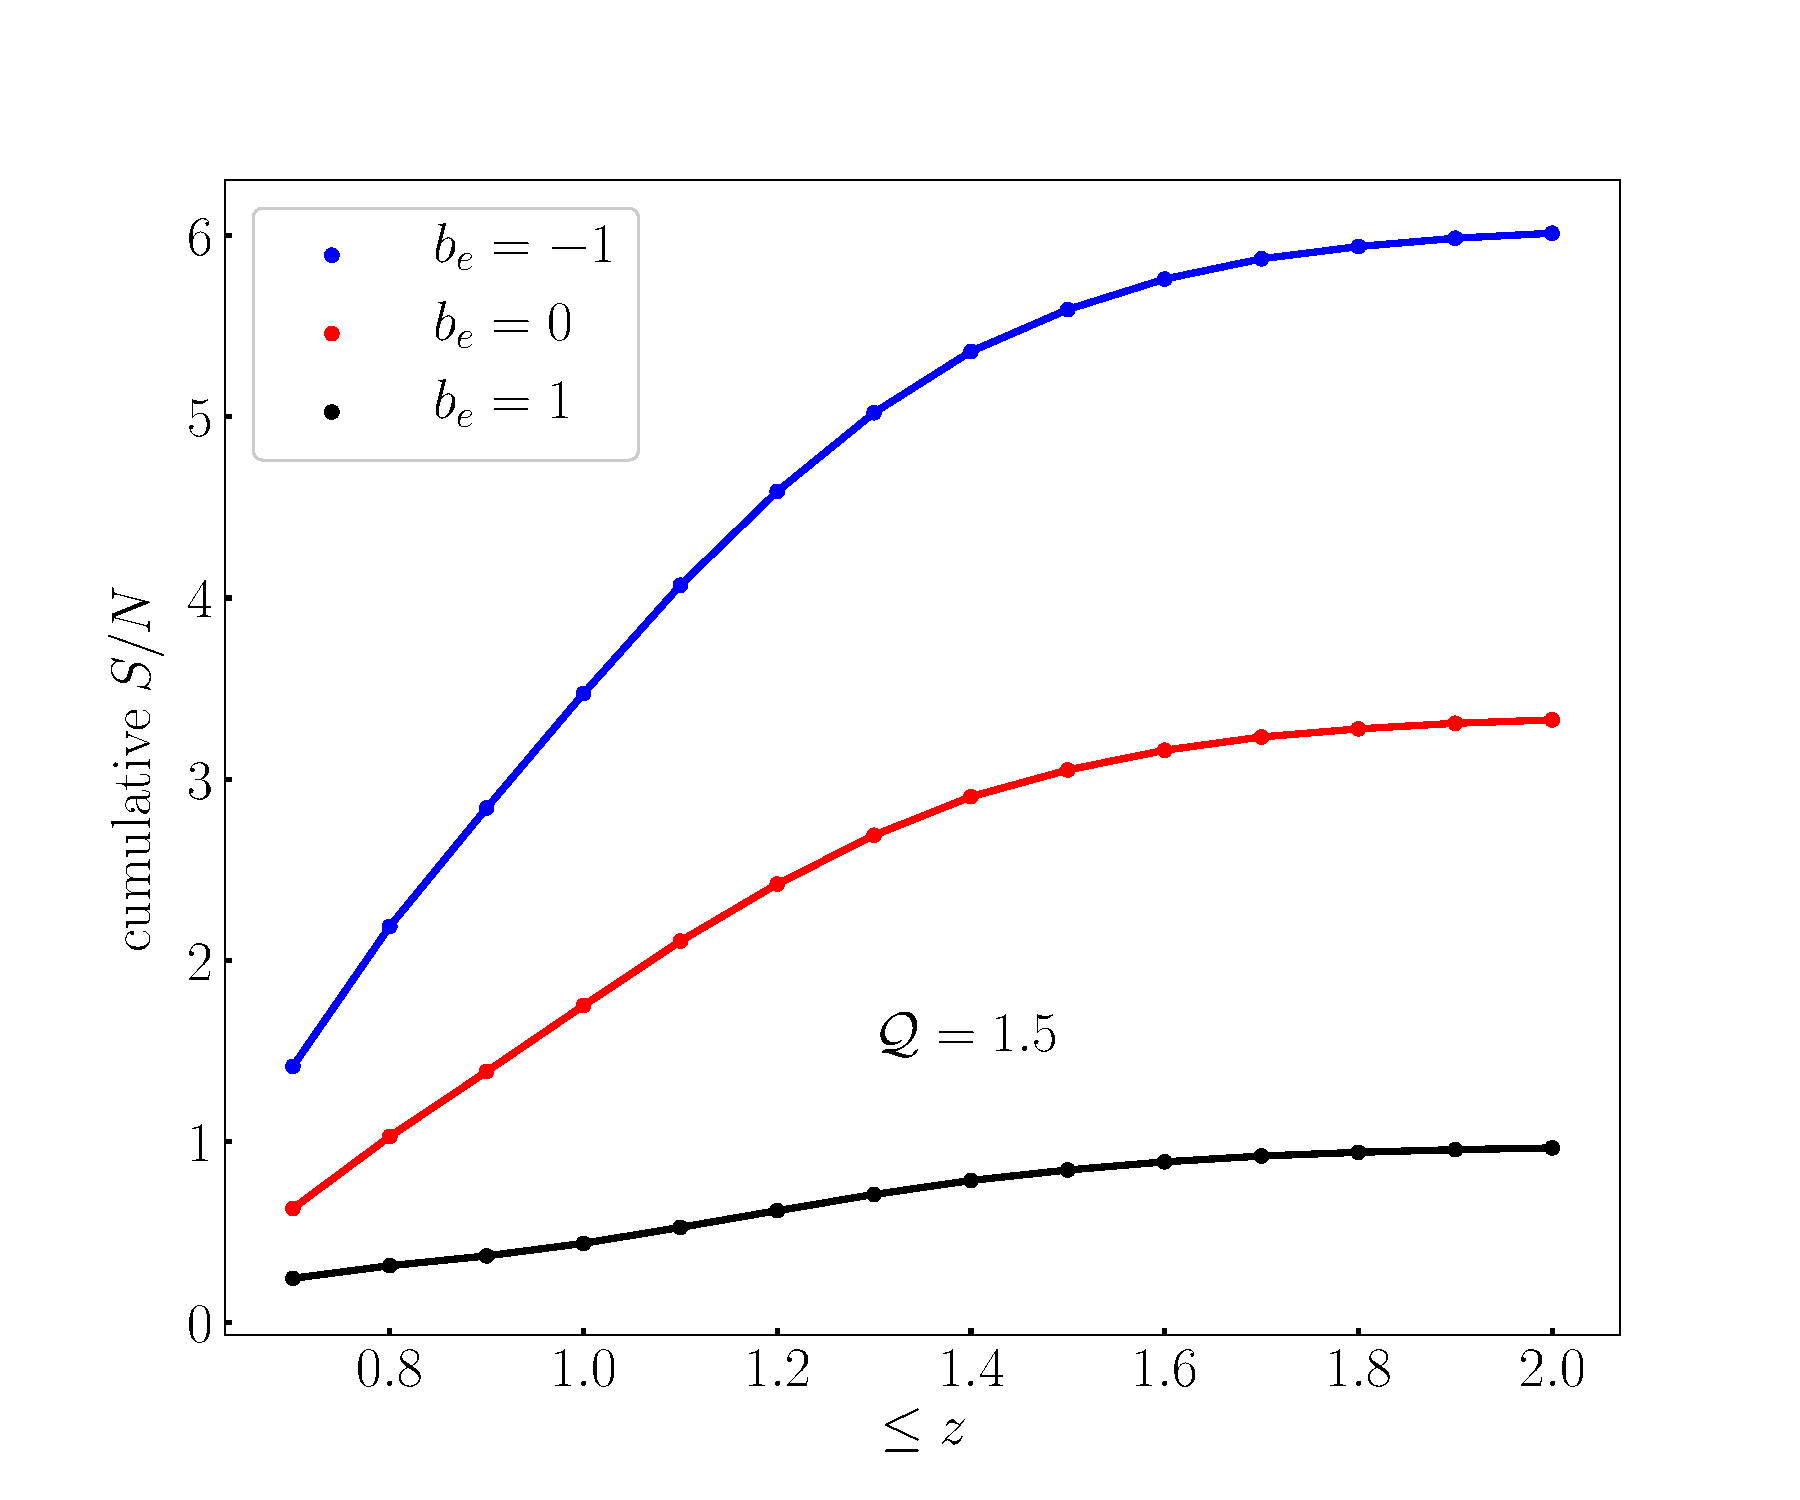
\includegraphics[width=7cm]{fig/cumulativeSnrdopplerQ1_5-eps-converted-to}
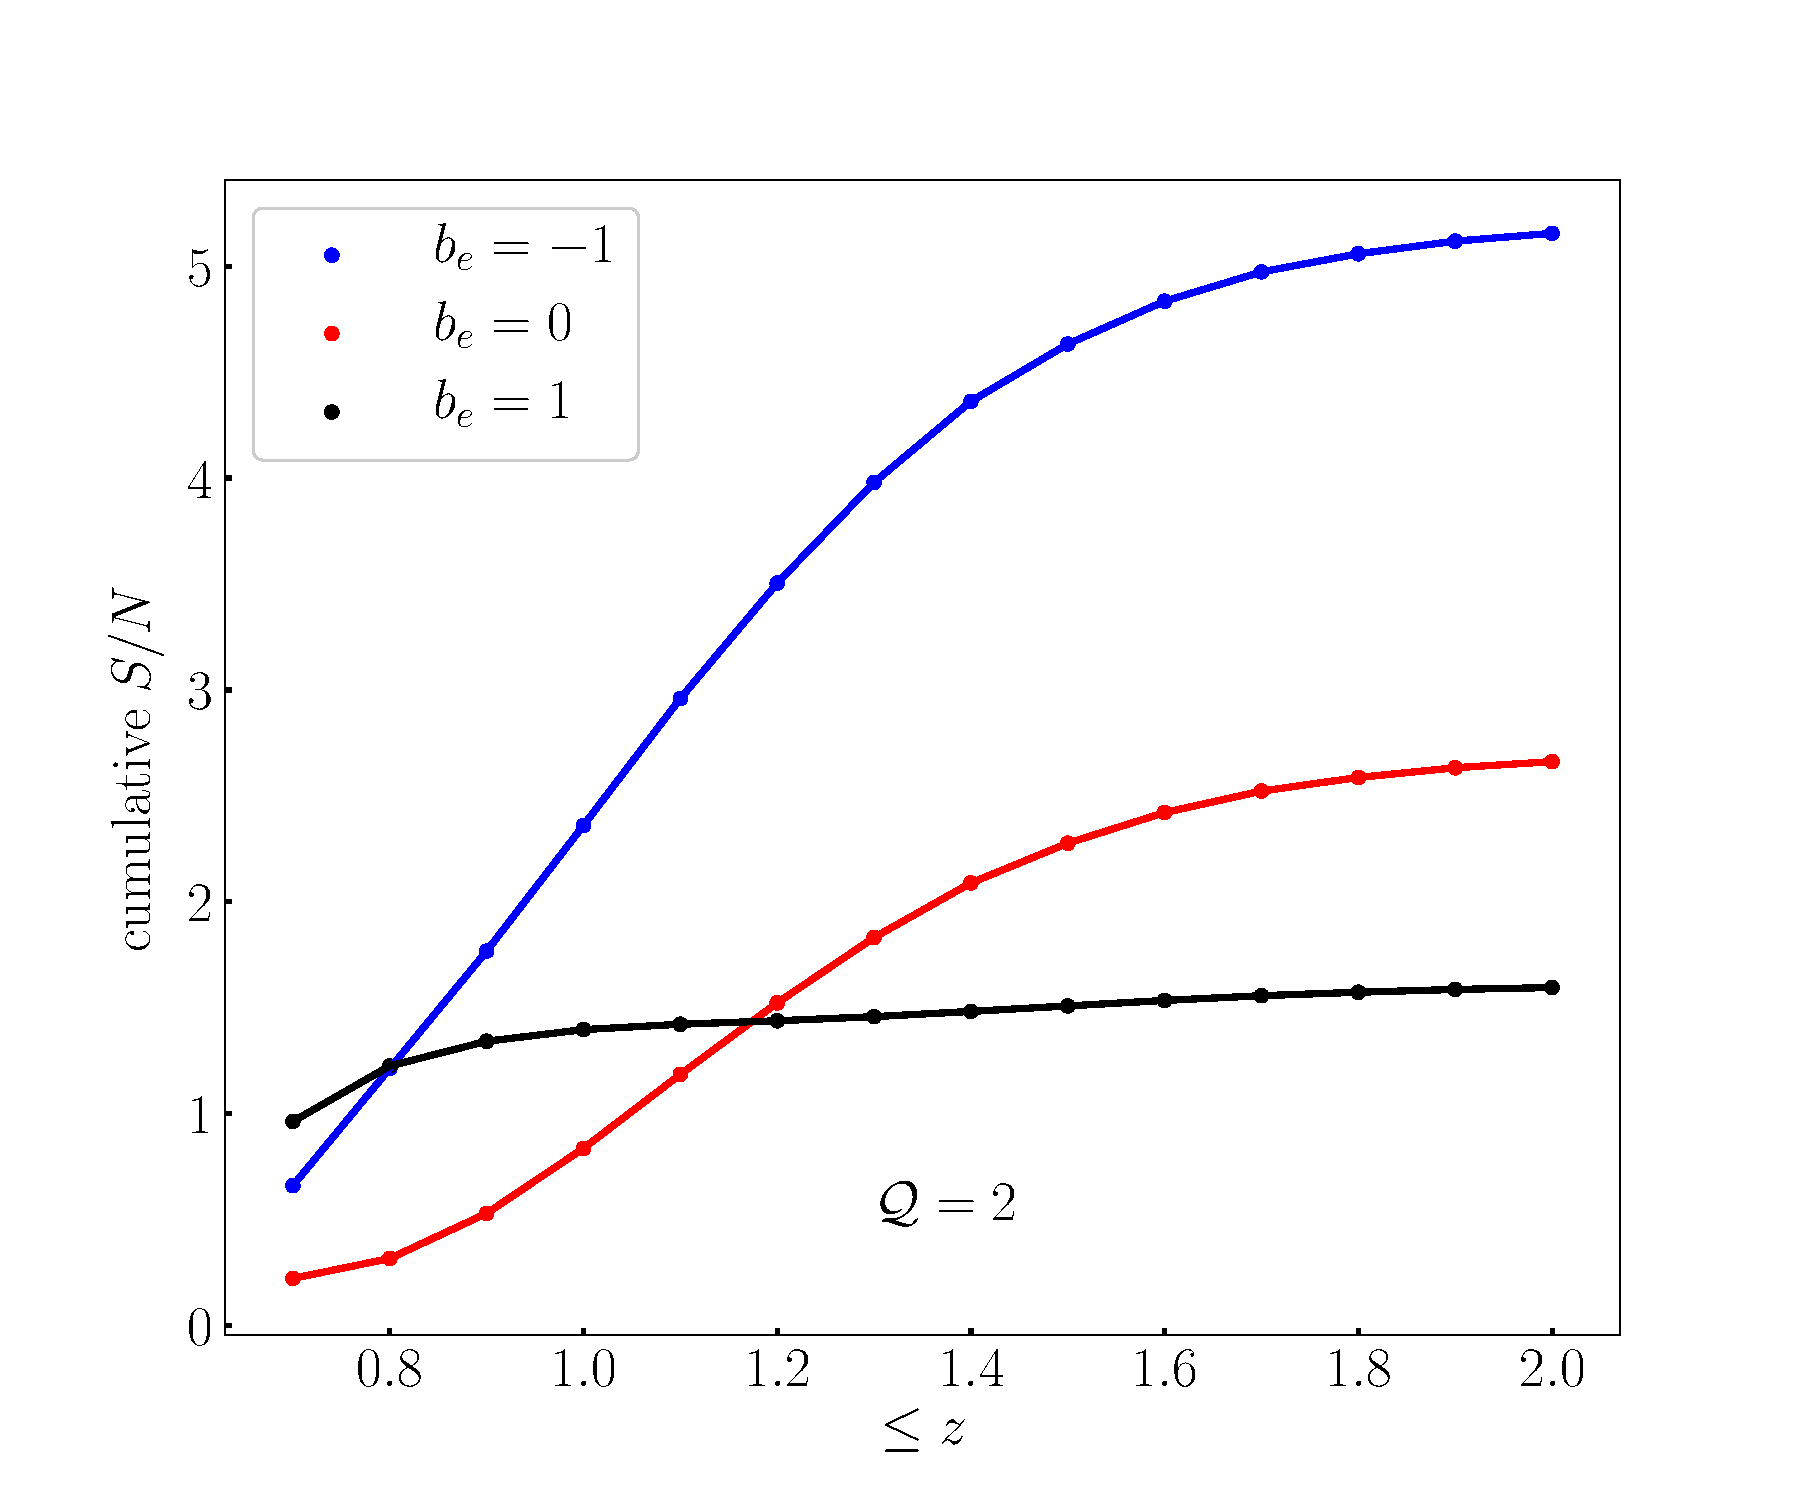
\includegraphics[width=7cm]{fig/cumulativeSnrdopplerQ2_0-eps-converted-to} 
\caption{Effect of changing ${\cal Q}$ and $b_e$ on relativistic cumulative SNR.} \label{fig1x}
\end{figure}


\subsection*{{Comparison with \cite{Jeong:2019igb}}}

In \cite{Jeong:2019igb},  
a significant number of terms is neglected in the relativistic second-order  galaxy number count contrast, $\delta_{g\mathrm{D}}^{(2)}$, given by our \eqref{dg2}. (Note that our  \eqref{dg2}, derived in \cite{Clarkson:2018dwn}, was independently confirmed by \cite{DiDio:2018zmk}). They have the first term, $A\, \bm{v}^{(2)}\!\!\cdot\bm{n}$, on the right of \eqref{dg2}.  In the second term, $2{C}(\bm{v}\cdot\bm{n})\,\delta$, they do not have the correct form of the coefficient $C$ -- they include only the first part, $b_1A$, of $C$ [see the right-hand side of \eqref{e26}]. All terms after the second term in \eqref{dg2} are omitted by \cite{Jeong:2019igb}. Note that none of the omitted terms is suppressed by a higher power of $k^{-1}$;  they all have the same scaling, i.e., $\propto (\cH/k)\,{(\delta)^2}$. In detail, they omit the following
terms:
\begin{align}
\delta_{g\mathrm{D}}^{(2)}({\mathrm{us}})- \delta_{g\mathrm{D}}^{(2)}(\mbox{{\cite{Jeong:2019igb}}}) &= 2\left[b_{1}f + \frac{b_1'}{\cH} 
+ 2\bigg(1-\frac{1}{{r} \cH}\bigg){\frac{\partial b_1}{\partial \ln{L}}\bigg|_{\mathrm{c}}} \right](\bm{v}\cdot\bm{n})\,\delta 
\\\nonumber
& 
+ \frac{2}{\cH}\left(4-2A-\frac{3}{2}\Omega_{m} \right)(\bm{v}\cdot\bm{n})\,\partial_r(\bm{v}\cdot\bm{n})\\
\nonumber
&
+ \frac{2}{\cH^2}\big[(\bm{v}\cdot\bm{n}) \,\partial_r^2\Phi-\Phi\, \partial_r^2 (\bm{v}\cdot\bm{n}) \big]
 - \frac{2}{\cH}\,\partial_r (\bm{v}\cdot\bm{v}) + 2 \frac{b_1}{\cH}\,\Phi\, \partial_r\delta \,. 
\end{align}